%!TEX root = ../../Main.tex

\subsection{Задача 2}
\frame{\subsectionpage}
\begin{frame}{Формулювання}

		Задача

		\begin{equation}\label{eq:problem2}
		\begin{cases}
			- \Delta u(x_1,x_2) + 10^5 u(x_1, x_2) = f(x_1,x_2), \\
			u|_\Gamma = 0 ,\\
			\Omega = \left[0;1\right] \times \left[0;1\right]
		\end{cases}
		\end{equation}

		Точний розв'язок
		\begin{equation}
			u(x,y) = x_1^{14}x_2(1-x_1)(1-x_2)+x_1 x_2^{14}(1-x_1)(1-x_2),
		\end{equation}

\end{frame}

\begin{frame}{Точний розв'язок}
		\begin{figure}[H]
			\centering
		    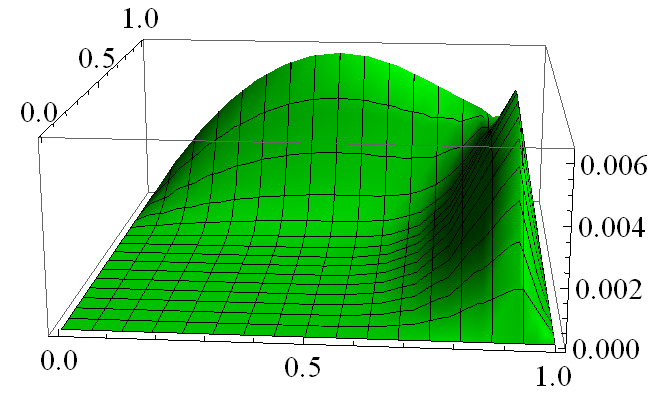
\includegraphics[width=0.8\textwidth]{problem2/ExactSolution}
		    \label{plot:problem1_exact}
		\end{figure}
\end{frame}

\begin{frame}[allowframebreaks]
	\frametitle<presentation>{Наближення}

	Граничну точність апроксимації на скінченному елементі - 7\%.
	Початкове розбиття - рівномірне на сітці 7x7


		\begin{figure}[H]
			 \begin{columns}
			 	\begin{column}{0.5\textwidth}
		     		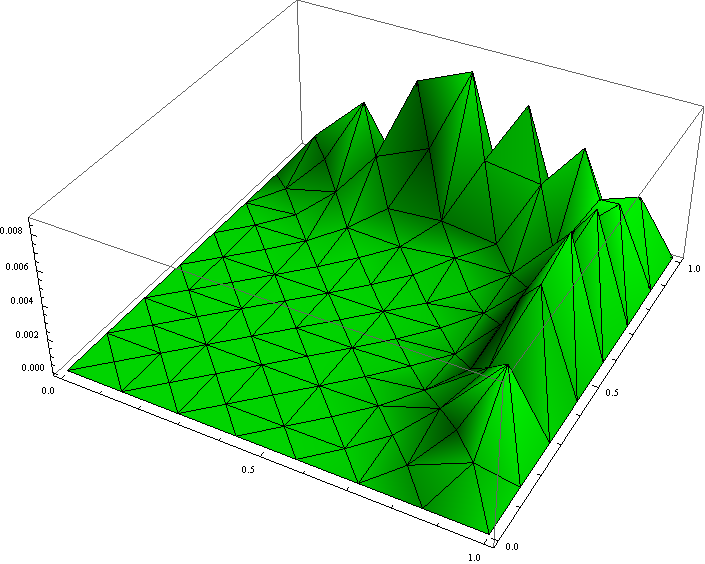
\includegraphics[width=\textwidth]{problem2/my/solutions/solution1}
		     	\end{column}
		     	\begin{column}{0.5\textwidth}
		     		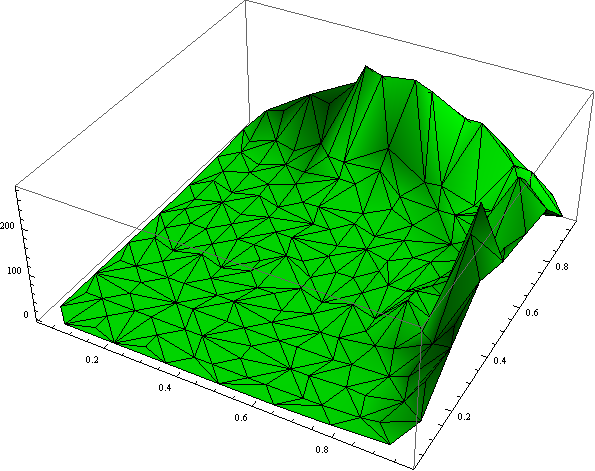
\includegraphics[width=\textwidth]{problem2/my/AEE/aee1}
		     	\end{column}
		     \end{columns}
		     \caption*{1-й крок. $N(h) = \nn{196}$.}
		\end{figure}
		%
		\begin{figure}[H]
			\begin{columns}
			 	\begin{column}{0.5\textwidth}
			 		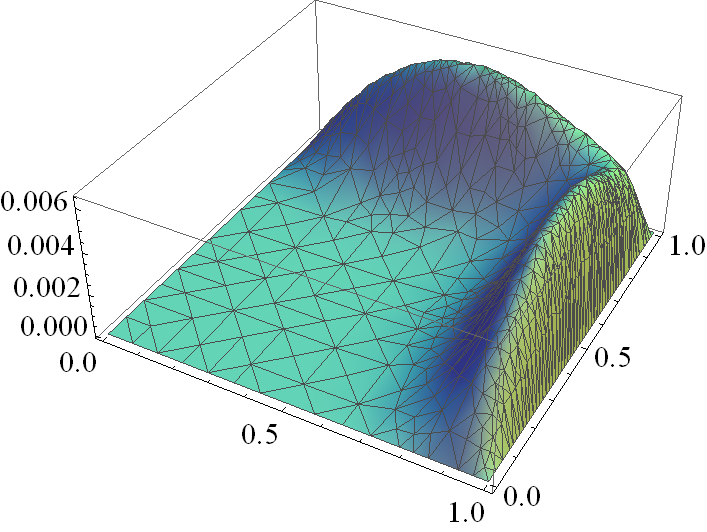
\includegraphics[width=\textwidth]{problem2/my/solutions/solution3}
			 	 \end{column}
			     \begin{column}{0.5\textwidth}
					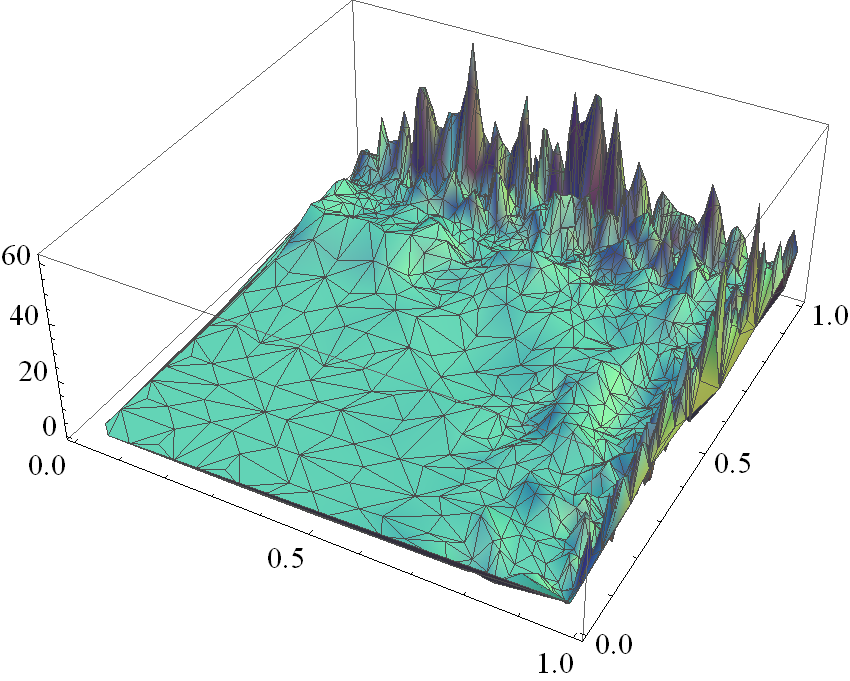
\includegraphics[width=\textwidth]{problem2/my/AEE/aee3}
			     \end{column}
		     \end{columns}
		     \caption*{3-й крок. $N(h) = \nn{1293}$.}
		\end{figure}
		%
		\begin{figure}[H]
			\begin{columns}
			 	\begin{column}{0.5\textwidth}
			 		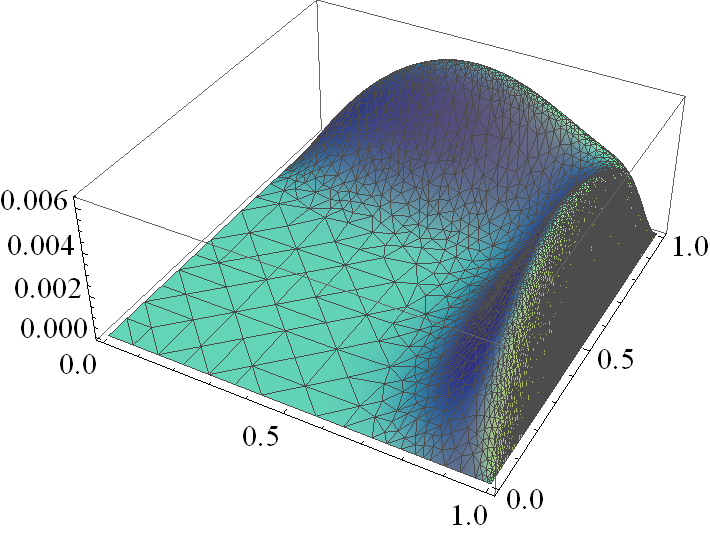
\includegraphics[width=\textwidth]{problem2/my/solutions/solution16}
			 	 \end{column}
			     \begin{column}{0.5\textwidth}
			     	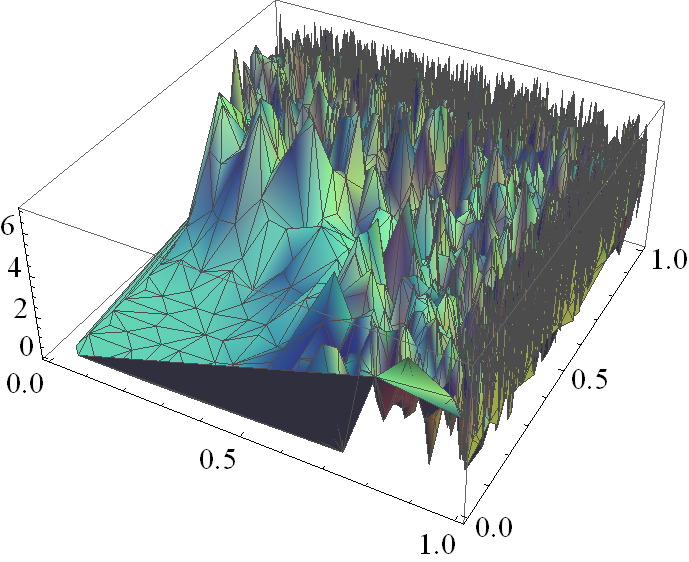
\includegraphics[width=\textwidth]{problem2/my/AEE/aee16}
			     \end{column}
		     \end{columns}
		     \caption*{16-й крок. $N(h) = \nn{9519}$.}
		\end{figure}
\end{frame}

\begin{frame}[allowframebreaks]
 	\frametitle<presentation>{Таблиця результатів}

 	\hspace{1cm}
 	\scriptsize{\pgfplotstabletypeset[col sep=comma,%
%
		columns={0,1,2,4,5,6,7,3},
		columns/0/.style={
			column name=\textnumero
		},
		columns/1/.style={
			column name=$N(h)$
		},
		columns/2/.style={
			column name=$M(h)$
		},
		columns/3/.style={
			column name=$\norm{e_h^\prime}\cdot 10^3$,
			preproc/expr={1000*##1}
		},
		columns/4/.style={
			column name=$\norm{e_h} \cdot 10^3$,
			preproc/expr={1000*##1}
		},
		columns/5/.style={
			column name=$\norm{e} \cdot 10^3$,
			preproc/expr={1000*##1}
		},
		columns/6/.style={
			column name=${P[u_h]}$,
			fixed,precision=2
		},
		columns/7/.style={
			column name=$\frac{\norm{e_h}}{\norm{e_h+u_h}}\%$
		},
		every head row/.style={before row=\toprule, after row=\midrule},
		every last row/.style={after row=\bottomrule},
		every nth row={1}{before row=\midrule},
		column type/.add={|}{|}
	]{include/8NumResults/problem2/my/errors/table.csv}
}
\end{frame}

\begin{frame}{Збіжність похибок}
	\begin{figure}[H]
		\centering
	    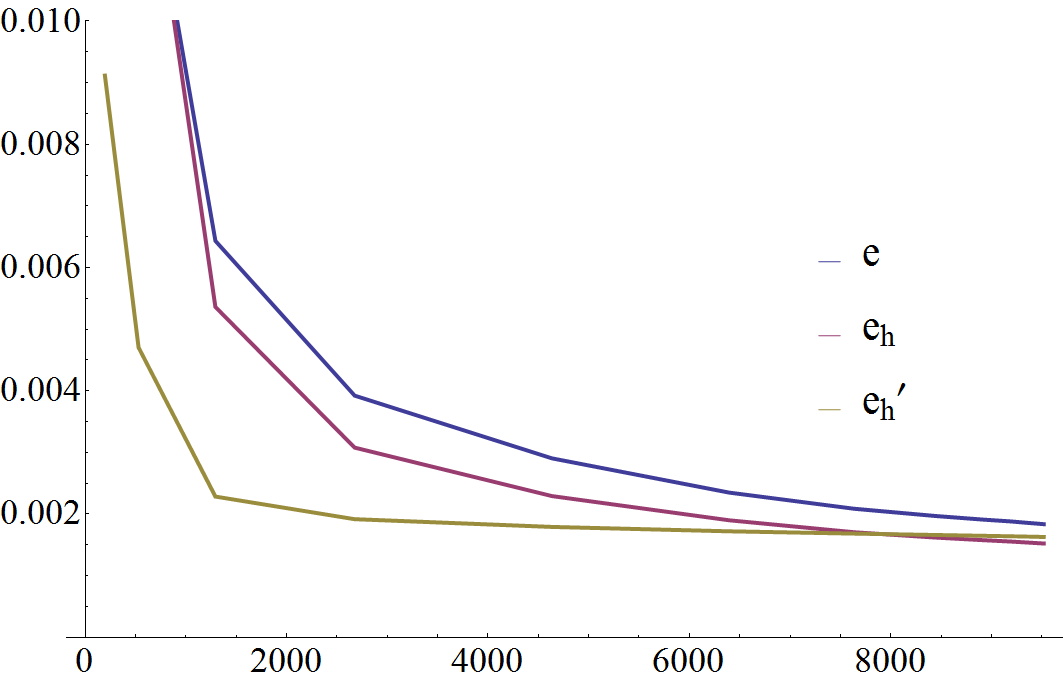
\includegraphics[height=0.8\textheight]{problem2/my/Plotnb}
	    \label{fig:p1_my_errors}
	\end{figure}
\end{frame}

\begin{frame}[allowframebreaks]
	{З оцінювачем Остапова-Шинкаренка}
	Якщо основу для адаптації беремо $e_h^\prime$
	\centering
	\scriptsize{\pgfplotstabletypeset[col sep=comma,%
		columns={0,1,2,3,5,6,7,4},
		columns/0/.style={
			column name=\textnumero
		},
		columns/1/.style={
			column name=$N(h)$
		},
		columns/2/.style={
			column name=$M(h)$
		},
		columns/3/.style={
			column name=$\norm{e_h^\prime} \cdot 10^3$,
			preproc/expr={1000*##1}
		},
		columns/4/.style={
			column name=$\norm{e_h} \cdot 10^3$,
			preproc/expr={1000*##1}
		},
		columns/5/.style={
			column name=$\norm{e} \cdot 10^3$,
			preproc/expr={1000*##1}
		},
		columns/6/.style={
			column name=${P[u_h]}$,
			fixed,precision=2
		},
		columns/7/.style={
			column name=$\frac{\norm{e_h^\prime}}{\norm{e_h^\prime+u_h}}\%$
		},
		every head row/.style={before row=\toprule, after row=\midrule},
		every last row/.style={after row=\bottomrule},
		every nth row={1}{before row=\midrule},
		column type/.add={|}{|}
	]{include/8NumResults/problem2/ost/errors/table.csv}}

\end{frame}

\begin{frame}{Збіжність похибок}
	\begin{figure}[H]
	 	\centering
	    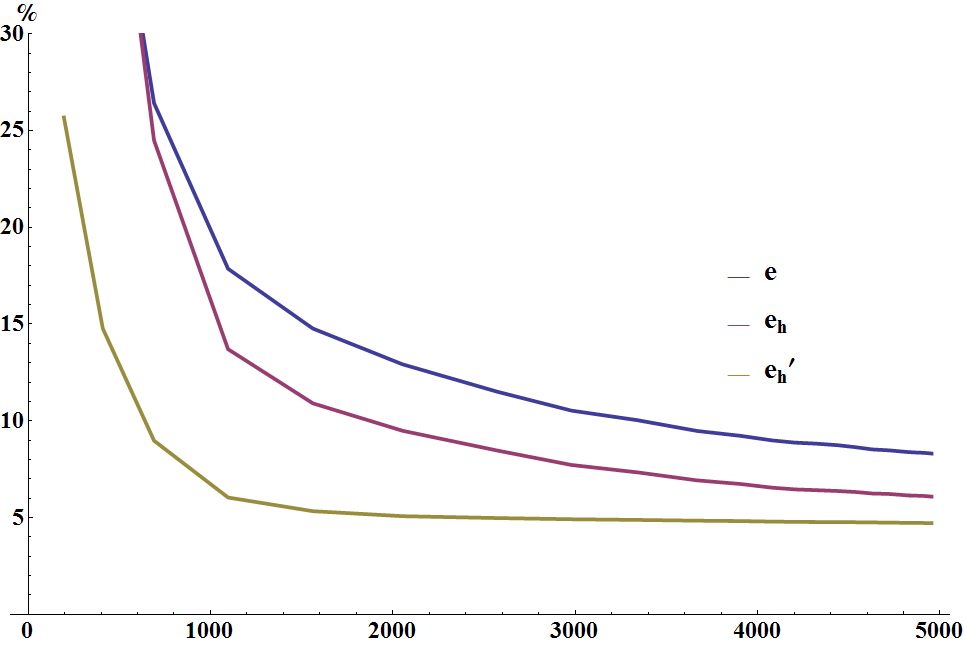
\includegraphics[width=0.8\textwidth]{problem2/ost/Plotnb}
	 \end{figure}
\end{frame}


\begin{frame}{Порівняння}
	\begin{figure}[H]
		\begin{columns}
		 	\begin{column}{0.5\textwidth}
		 		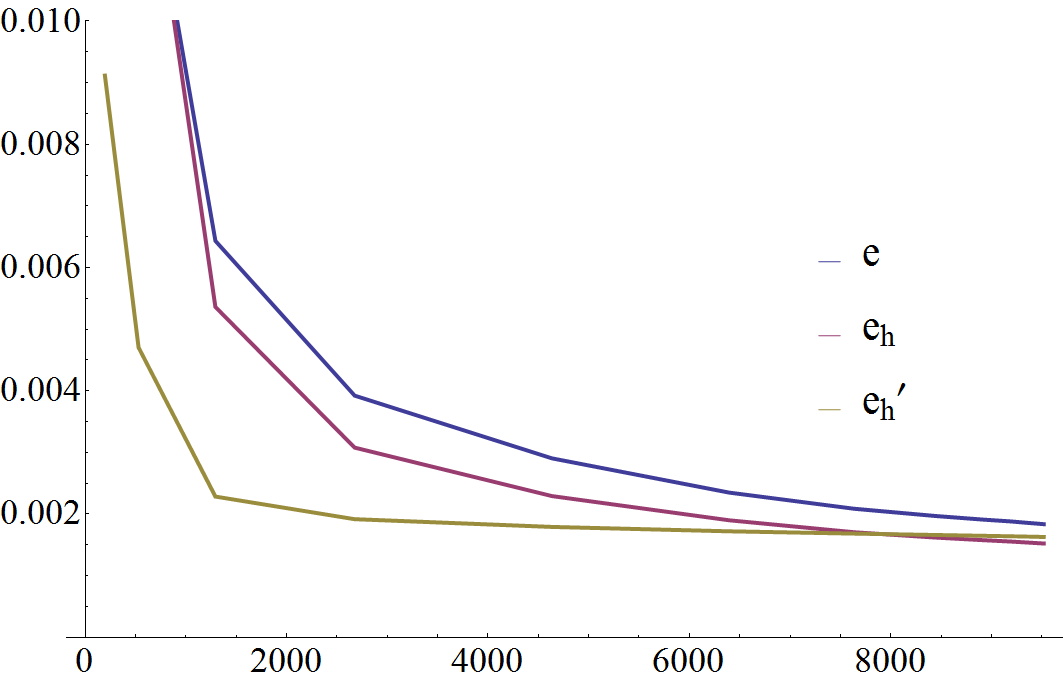
\includegraphics[width=\textwidth]{problem2/my/Plotnb}
		 	 \end{column}
		     \begin{column}{0.5\textwidth}
		     	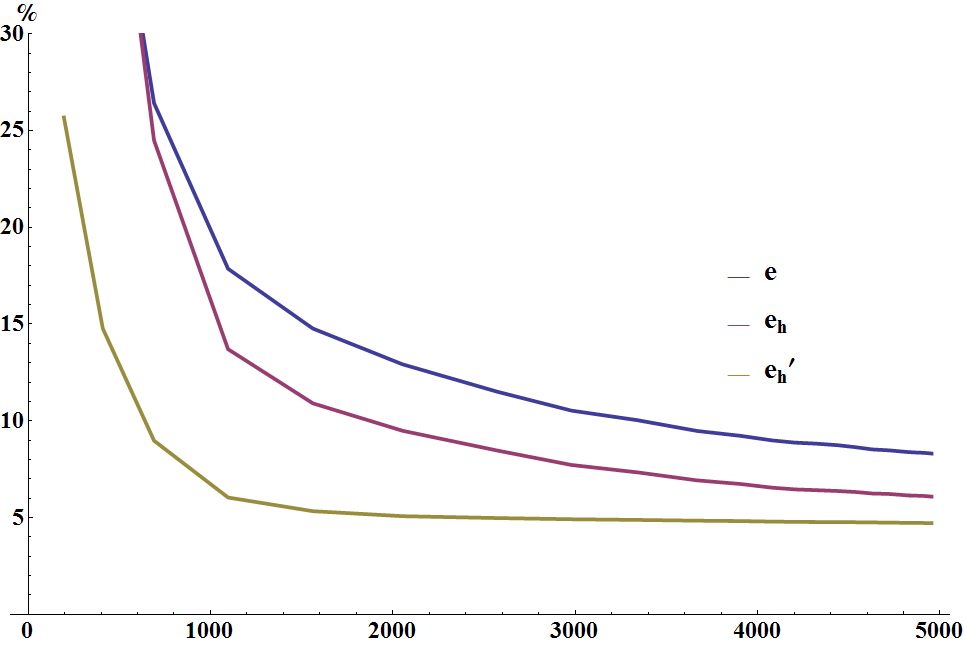
\includegraphics[width=\textwidth]{problem2/ost/Plotnb}
		     \end{column}
		\end{columns}
	\end{figure}
\end{frame}
